\chapter{Instrukcja obsługi}
\section{Uruchomienie aplikacji}
Poniżej przedstawiamy krótką instrukcję obsługi systemu przez nas zbudowanego.
Instrukcja dotyczy części webowej. Niestety nie udało nam się uruchomić schedulera z linii
poleceń, więc nie opisujemy co zrobić by system działał razem z nim.
\\
Do uruchomienia aplikacji webowej potrzebujemy uruchomiony serwer PHP oraz interpreter Pythona.
Całą strukturę katalagów przenosimy do folderu ze stronami naszego serwera PHP (tak, aby móc
się do niego dostać poprzez adres \texttt{http://localhost/nazwa-katalogu}).
\\
Aplikację powinno się uruchamiać w przeglądarce wspierającej HTML5. My testowaliśmy ją w przeglądarce
Google Chrome (v. 19), w której sprawowała się bardzo dobrze.
\\
Jeśli wszystko pójdzie sprawnie powinniśmy ujrzeć ekran powitalny. Po najechaniu myszką w napis
\textbf{Web Dispatch Rider} pojawi nam się menu z trzema pozycjami na liście.

\section{Dodawanie zadania}
W tym widoku użytkownik może dodać nowe zadanie do systemu poprzez zdefiniowanie jego nazwy
oraz wybranie odpowiednich plików dotyczących zadania. System nie pozwoli na wysłanie plików
w niepoprawnym formacie, bądź w sytuacji, w której nie zostaną podane wszystkie pliki
przez użytkownika. W przypadku poprawnego wykonania się operacji przesłania plików
użytkownik otrzyma na ten temat stosowny komunikat, a skrypt Pythonowski utworzy na serwerze
plik w JavaScripcie ze współrzędnymi odzwierciedlającymi mapkę danego zadania.

\section{Zadania w trakcie}
W tym miejscu użytkownik może podejrzeć listę zadań, które czekają w kolejce na bycie przetworzonym
przez zewnętrzny moduł Dispatch Ridera. Do momentu rozpoczęcia przetwarzania użytkownik ma możliwość
edycji tych plików zgodnie z własną wolą. Kiedy system przejmie zadanie, wówczas edycja nie jest już
możliwa.

\section{Zadania obliczone}
Tutaj znajduje się lista zadań gotowych do obejrzenia przez użytkownika. Może on obejrzeć graf dotyczący
danego zadania lub usunąć zadanie. Dane te są dostępne dla użytkownika cały czas. W przypadku gdy
zadanie jest jeszcze liczone, bądź czeka w kolejce użytkownikowi wyświetla się tylko mapka dotycząca danego zadania.

\subsection{Wyświetlanie grafu}
Użytkownik wybierając podgląd grafu danego zadania może zobaczyć jego mapkę oraz przebieg tras wszystkich kierowców.
Mapa pokazuje miejsca z podziałem na miejsca dostarczenia przesyłek i miejsca ich odbioru.
\newline

\begin{center}
\begin{figure}[H]
\centering
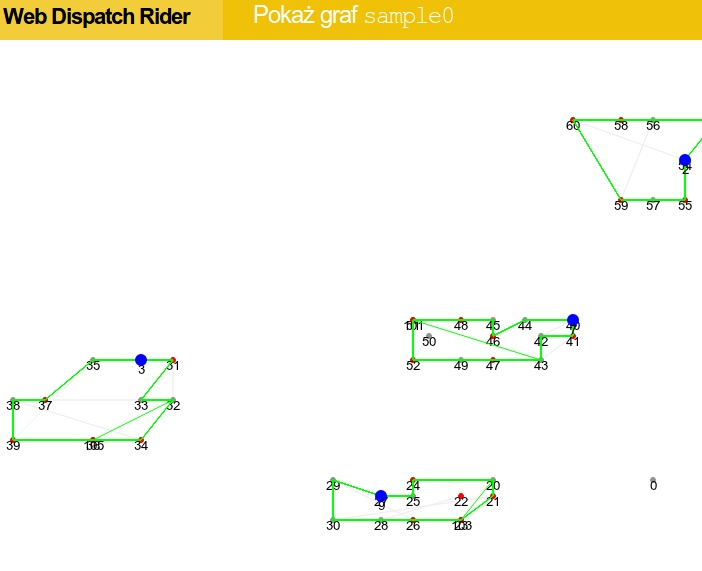
\includegraphics[scale=0.5]{imgs/graf.jpg}
\caption{Diagram komponentów systemu}
\label{fig:diagram_komponentow}
\end{figure}
\end{center}

\subsection{Zmiana sposobu wyświetlania grafu}
W dokumentacji należy się również słowo wyjaśnienia odnośnie sposobu wyświetlania grafu.
Na początku semestru uznaliśmy, że skorzystamy z gotowych bibliotek JavaScriptowych analizując je
i wybierając naszym zdaniem najlepszą. Wówczas jednak nie byliśmy do końca świadomi grafu jaki powinniśmy
uzyskać w budowanym przez nas systemie. Biblioteka, którą wybraliśmy nie umożliwiała nam rysowanie grafów/węzłów
w określonych przez nas miejscach ekranu. W związku z tym postanowiliśmy bliżej zaznajomić się z technologią Canvas,
którą dostarcza HTML5. Udało nam się tę znajomość zakończyć pozytywnie i uzyskać poruszający się w przeglądarce graf.